\documentclass{beamer}

\usepackage[utf8]{inputenc}
\usepackage{amsmath}
\usepackage{amsfonts}
\usepackage{amssymb}
\usepackage{graphicx}
\usepackage{tikz}
\usepackage{hyperref}

\graphicspath{{../}{./}{../images/}{./images/}}

% ===== KCPC clean theme =====
\usetheme{default}
\useinnertheme{rectangles}
\useoutertheme{default}

\setbeamertemplate{navigation symbols}{}

% --- Colours ---
\definecolor{kcpc-bg}{RGB}{250,250,250}
\definecolor{kcpc-text}{RGB}{20,20,20}
\definecolor{kcpc-muted}{RGB}{90,90,90}
\definecolor{kcpc-red}{RGB}{176,0,0}

\setbeamercolor{background canvas}{bg=kcpc-bg}
\setbeamercolor{normal text}{fg=kcpc-text}
\setbeamercolor{frametitle}{fg=kcpc-text,bg=kcpc-bg}
\setbeamercolor{title}{fg=kcpc-text}
\setbeamercolor{subtitle}{fg=kcpc-muted}
\setbeamercolor{structure}{fg=kcpc-red}

\setbeamerfont{title}{series=\bfseries,size=\Large}
\setbeamerfont{frametitle}{series=\bfseries,size=\large}

\setlength{\parskip}{0.4em}

\setbeamertemplate{itemize item}{$\rightarrow$}
\setbeamertemplate{itemize subitem}{$\rightarrow$}

\setbeamertemplate{headline}{
    \vspace{0.2cm}
    \hspace{0.2cm}
    \textcolor{kcpc-muted}{\small\insertsection}
    \hfill
}

\setbeamertemplate{footline}{
    \hspace{0.2cm}
    \textcolor{kcpc-muted}{\small KCPC}
    \hfill
    \vspace{0.3cm}
}

\setbeamertemplate{background}{
    \begin{tikzpicture}[remember picture,overlay]
        \node[
            opacity=0.035,
            at=(current page.center)
        ] {
            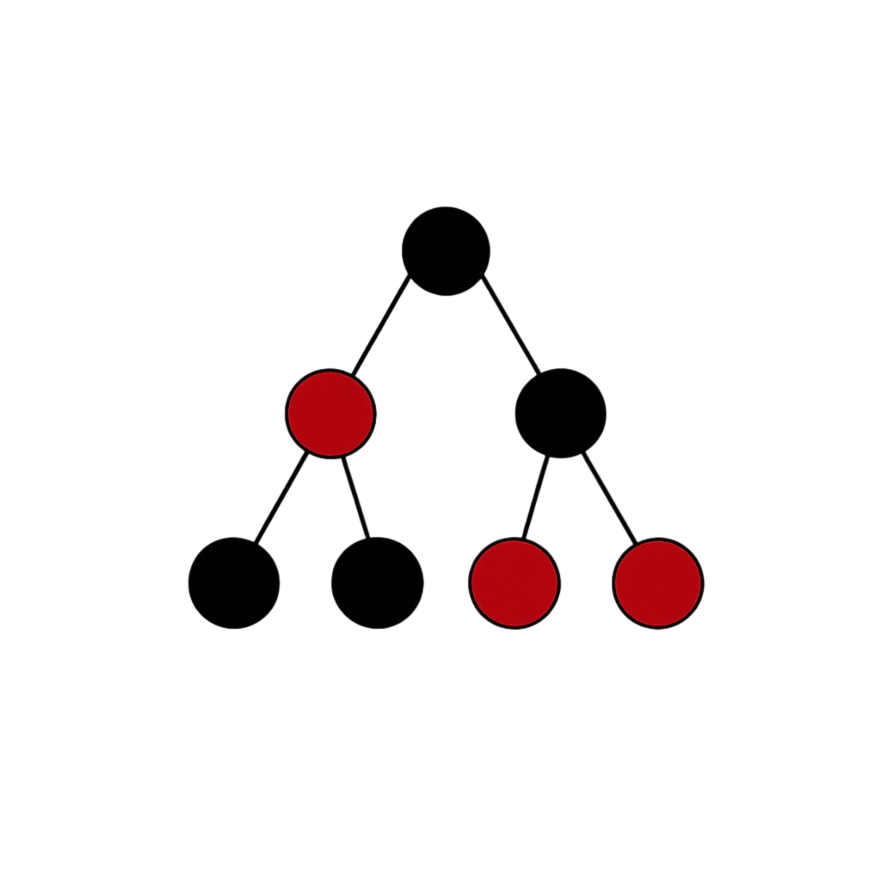
\includegraphics[width=0.55\paperwidth]{kcpc-logo.png}
        };
    \end{tikzpicture}
}

\AtBeginSection[]{
    \begin{frame}[plain]
        \vfill
        \centering
        {\Large\bfseries \insertsection}
        \vfill
    \end{frame}
}

\hypersetup{colorlinks=true,linkcolor=kcpc-red,urlcolor=kcpc-red}

\title{Some Techniques for Investigation}
\subtitle{More sophistication than banging our heads at problems}
\author{King's Competitive Programming Club}
\date{Workshop 2}

\begin{document}

% Slide 1
\begin{frame}[plain]
    \titlepage
\end{frame}

% Slide 2
\begin{frame}{Workshop Agenda}
    \begin{itemize}
        \item What did we learn last week?
        \item Psychological strategies
        \item Strategies for investigating problems
        \item Some more problems and homework
        \item Final messages
    \end{itemize}
\end{frame}

% Slide 3
\begin{frame}[plain]
    \vfill
    \centering
    {\Large\bfseries Oh, and also:}
    \vfill
\end{frame}

% Slide 4
\begin{frame}{Our Socials}
    \centering
    \begin{columns}[c]
        \column{0.33\textwidth}
        \centering
        
\includegraphics[width=\textwidth]{insta.png}
        \par\vspace{0.4em}
        Instagram

        \column{0.33\textwidth}
        \centering
        
\includegraphics[width=\textwidth]{whatsapp.png}
        \par\vspace{0.4em}
        WhatsApp

        \column{0.33\textwidth}
        \centering
        
\includegraphics[width=\textwidth]{discord.png}
        \par\vspace{0.4em}
        Discord
    \end{columns}
\end{frame}

% Section 1
\section{What did we learn last week?}

\begin{frame}{What did we learn last week?}
    \begin{itemize}
        \item We got our hands dirty.
        \pause
        \item Stay loose and experiment.
        \pause
        \item Plug in lots of numbers.
        \pause
        \item Keep playing around until you see a pattern.
        \pause
        \item Then, play around some more, and try to figure out why the pattern you see is happening.
    \end{itemize}
\end{frame}

\begin{frame}{What did we learn last week?}
    \begin{itemize}
        \item We saw ``problems'' not ``exercises''.
        \pause
        \item \textbf{Exercises} are never puzzling, for it is always immediately clear how to proceed.
        \pause
        \item A \textbf{problem} is a question that cannot be answered immediately.
        \pause
        \item Problems are often open-ended, paradoxical, and sometimes unsolvable, and require investigation before one can come close to a solution.
    \end{itemize}
\end{frame}

% Section 2
\section{Psychological strategies}

\begin{frame}{Psychological strategies}
    \begin{itemize}
        \item We are not promising improvement in \textbf{solving} problems. That will come with time.
        \pause
        \item But first you have to learn to \textbf{really} work.
        \pause
        \item \textbf{Mental Toughness}
        \pause
        \item \textbf{Creativity}
    \end{itemize}
\end{frame}

\begin{frame}{Psychological strategies $>$ Mental toughness}
    \begin{itemize}
        \item Don’t give up, nor bang your head on the wall.
        \pause
        \item Vary each attempt.
        \pause
        \item But: learn to know when to give up (\textbf{temporarily}!)
    \end{itemize}
\end{frame}

\begin{frame}{Psychological strategies $>$ Creativity}
    \begin{itemize}
        \item Be the magic.
        \pause
        \item Remember: Ants on a ruler problem
        \pause
        \item From: ``Wow! How did she think of that? I could never have done it.''
        \pause
        \item To: ``Nice idea! It’s similar to ones I’ve had. Let’s put it to work!''
        \pause
        \item Stay loose.
        \pause
        \item Cultivate a sort of mental peripheral vision.
    \end{itemize}
\end{frame}

\begin{frame}{Psychological strategies $>$ Creativity}
    Pat wants to take a 1.5-meter-long sword onto a train, but the conductor won’t allow it as carry-on luggage. And the baggage person won’t take any item whose greatest dimension exceeds 1 meter.
    \pause
    \vspace{1em}

    \textbf{What should Pat do?}
\end{frame}

\begin{frame}{Psychological strategies $>$ Creativity}
    \begin{columns}[c]
        \begin{column}{0.6\textwidth}
            We have two polyhedra (i.e., solids with polygonal faces), all of whose edges have length 1: a pyramid with a square base, and a tetrahedron (a tetrahedron is composed of four triangular faces).
            \pause
            \vspace{0.5em}

            Suppose we glue the two polyhedra together along a triangular face (so that the attached faces exactly overlap).
            \pause
            \vspace{0.5em}

            \textbf{How many faces does the new solid have?}
        \end{column}
        \begin{column}{0.38\textwidth}
            \centering
            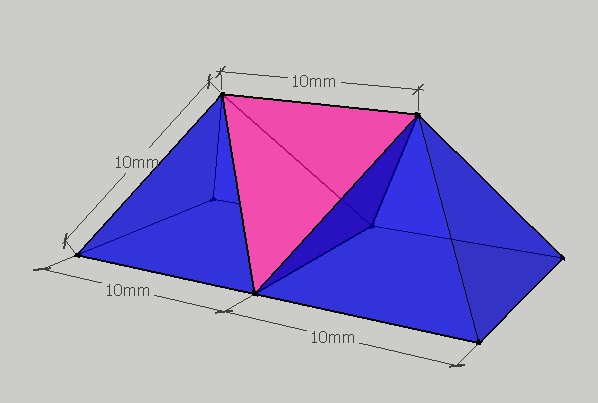
\includegraphics[width=\linewidth]{polyhedra.png}
        \end{column}
    \end{columns}
\end{frame}

% Section 3
\section{Strategies for investigating problems}

\begin{frame}{Strategies for investigating problems}
    \begin{itemize}
        \item Simple ideas, but will allow you to make encouraging progress.
        \pause
        \item \textbf{The investigation:} Discover what is going on.
        \begin{itemize}
            \item Go make some observations.
            \item List them out.
        \end{itemize}
        \pause
        \item \textbf{Argument:} Convince yourself (or others) of your discoveries.
        \pause
        \item There is an easy way in competitive programming\dots
    \end{itemize}
\end{frame}

\begin{frame}{Strategies for investigating problems $>$ Wishful thinking/Make it easier}
    \begin{itemize}
        \item Ask yourself, ``What is it about the problem that makes it hard?'' Then, make the difficulty disappear!
        \pause
        \item You may not be able to do this \textbf{legally}, but who cares?
        \pause
        \item Eliminating the hard part of a problem, even temporarily, will allow you to have some fun and raise your confidence.
        \pause
        \item Make some progress with its easier cousin!
    \end{itemize}
\end{frame}

\begin{frame}{Strategies for investigating problems $>$ Wishful thinking/Make it easier}
    The sequence $a_0, a_1, a_2, \dots$ satisfies
    \[ a_{m+n} + a_{m-n} = \frac{1}{2}(a_{2m} + a_{2n}) \]
    for all non-negative integers $m$ and $n$ with $m \ge n$.
    \pause
    \vspace{0.8em}

    If $a_1 = 1$, determine $a_{6767}$.
\end{frame}

\begin{frame}{Strategies for investigating problems $>$ Wishful thinking/Make it easier}
    Let $\mathbb{N}$ denote the natural numbers $1, 2, 3, 4, \dots$ Consider a function $f$ that satisfies:
    \[ f(1) = 1, \quad f(2n) = f(n), \quad \text{and} \quad f(2n + 1) = f(2n) + 1 \]
    for all $n \in \mathbb{N}$.
    \pause
    \vspace{0.8em}

    Find a nice simple algorithm for $f(n)$. Your algorithm should be a single sentence long, at most.
\end{frame}

\begin{frame}{Strategies for investigating problems $>$ Induction}
    \begin{itemize}
        \item This is a very powerful method for proving assertions that are ``indexed'' by integers.
        \pause
        \item Prove the base case.
        \pause
        \item Find a direct assertion from $n \to n + 1$.
    \end{itemize}
\end{frame}

\begin{frame}{Strategies for investigating problems $>$ Induction}
    Prove that if $n$ is an integer greater than 3, then
    \[ n! > 2^n \]
\end{frame}

\begin{frame}{Strategies for investigating problems $>$ Induction}
    \begin{itemize}
        \item But you might say: ``This is competitive \textbf{programming}, not competitive mathematics.''
        \pause
        \item In fact, (backwards) induction is used in a very powerful method called \textbf{dynamic programming}, which we will learn in time!
    \end{itemize}
\end{frame}

\begin{frame}{Strategies for investigating problems $>$ Draw a picture/Recast/Change POV}
    \begin{itemize}
        \item Awareness that problems can and should be reformulated in different ways.
        \pause
        \item Open your mind to other ways of reinterpreting problems!
        \pause
        \item Sometimes a problem is hard only because we choose the ``wrong'' point of view. Spending a few minutes searching for the ``natural'' point of view can pay big dividends.
    \end{itemize}
\end{frame}

\begin{frame}{Strategies for investigating problems $>$ Draw a picture/Recast/Change POV}
    Remove the two diagonally opposite corner squares of a chessboard.
    \pause
    \vspace{0.8em}

    Is it possible to tile this shape with thirty-one $2 \times 1$ ``dominos?''
    \vspace{0.8em}

    (In other words, every square is covered and no dominos overlap.)
\end{frame}

\begin{frame}{Strategies for investigating problems $>$ Draw a picture/Recast/Change POV}
    \begin{columns}[c]
        \begin{column}{0.6\textwidth}
            Once again, you can easily use induction to prove the very cool fact that the sum of the first $n$ perfect cubes is equal to the square of the $n$-th triangular number:
            \[ \sum_{i=1}^n i^3 = \left(\sum_{i=1}^n i\right)^2 \]
            \pause
            \textbf{Can you do it with a picture, instead?}
        \end{column}
        \begin{column}{0.38\textwidth}
            \centering
            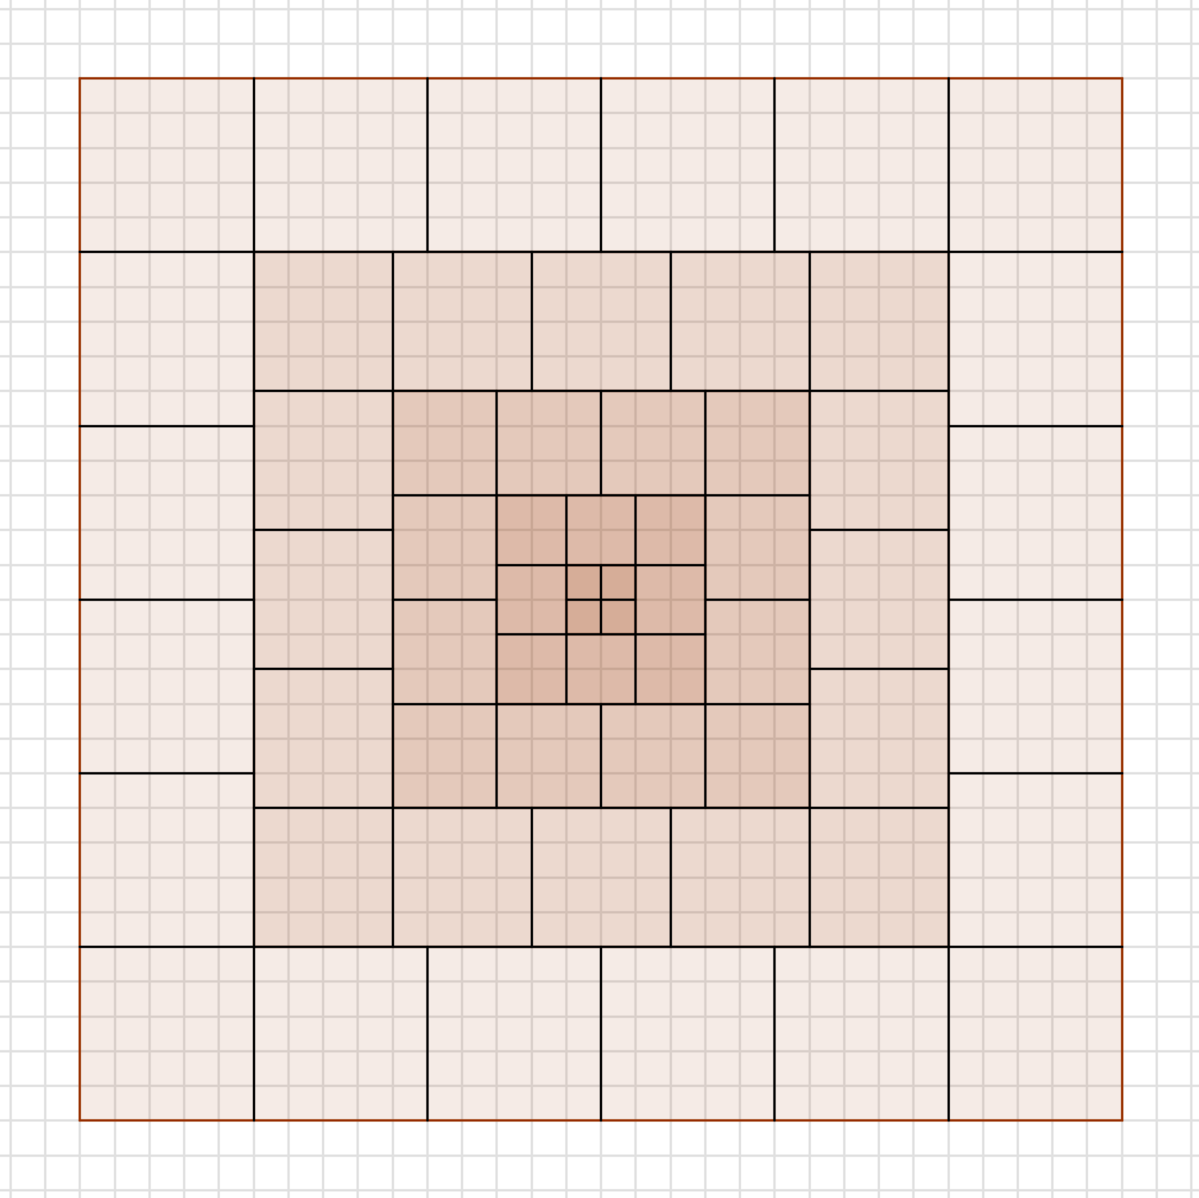
\includegraphics[width=\linewidth]{cubes.png}
        \end{column}
    \end{columns}
\end{frame}

\begin{frame}{Strategies for investigating problems $>$ Draw a picture/Recast/Change POV}
    What is the first time after 12 o’clock at which the hour and minute hands meet?
    \pause
    \vspace{0.8em}

    This is an amusing and moderately hard algebra exercise, well worth doing if you never did it before.
    \pause
    \vspace{0.8em}

    However, this problem can be solved in a few seconds in your head if you avoid messy algebra and just consider the ``natural'' point of view. Go for it!
  \end{frame}

\begin{frame}{Strategies for investigating problems $>$ Symmetry}
    \begin{itemize}
        \item We call an object symmetric if there are one or more non-trivial ``actions'' that leave the object unchanged. We call the actions that do this the symmetries of the object.
        \pause
        \item A square is symmetric with respect to reflection about a diagonal.
        \pause
        \item A circle has infinitely many symmetries.
    \end{itemize}
\end{frame}

\begin{frame}{Strategies for investigating problems $>$ Symmetry}
    \begin{columns}[c]
        \begin{column}{0.6\textwidth}
            A square is inscribed in a circle that is inscribed in a square.
            \pause
            \vspace{1em}

            \textbf{Find the ratio of the areas of the two squares.}
        \end{column}
        \begin{column}{0.38\textwidth}
            \centering
            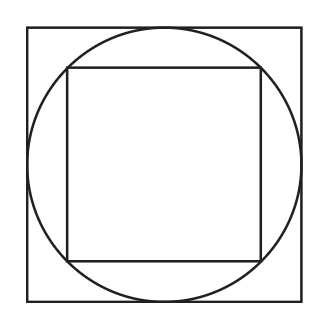
\includegraphics[width=0.9\linewidth]{sym.png}
        \end{column}
    \end{columns}
\end{frame}

\begin{frame}{Strategies for investigating problems $>$ Symmetry}
    \begin{columns}[c]
        \begin{column}{0.6\textwidth}
            Your cabin is two miles due north of a stream that runs east-west. Your grandmother’s cabin is located 12 miles west and one mile north of your cabin.
            \pause
            \vspace{0.5em}

            Every day, you go from your cabin to Grandma’s, but first visit the stream (to get fresh water for Grandma).
            \pause
            \vspace{0.5em}

            \textbf{What is the length of the route with minimum distance?}
        \end{column}
        \begin{column}{0.38\textwidth}
            \centering
            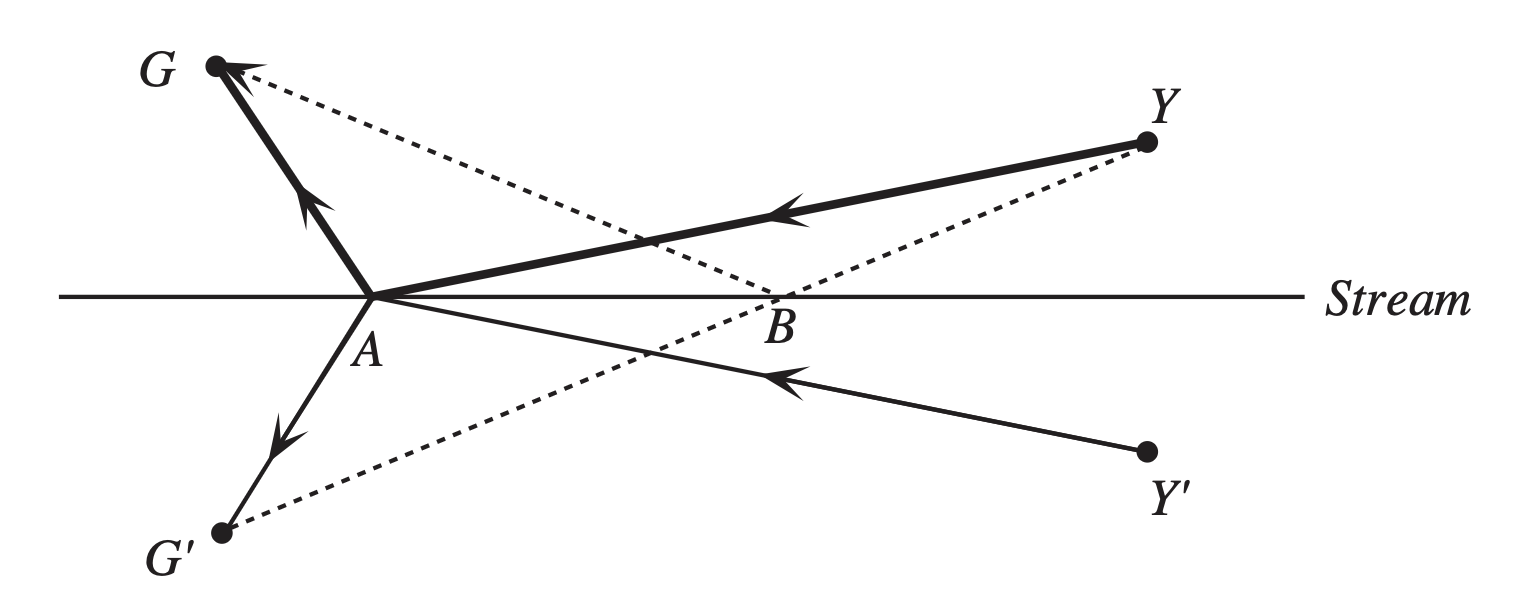
\includegraphics[width=\linewidth]{grandma.png}
        \end{column}
    \end{columns}
\end{frame}

\begin{frame}{Strategies for investigating problems $>$ The extreme principle}
    \begin{itemize}
        \item If possible, assume that the elements of your problem are ``in order.'' Focus on the ``largest'' and ``smallest'' elements, as they may be constrained in interesting ways.
        \pause
        \item \textbf{Strategy-ception: Argument by contradiction.}
        \pause
        \item Assume that whatever you wish to prove is not true. Then look at the minimal (or maximal) element and develop an argument that creates a smaller (or larger) element, which is the desired contradiction.
    \end{itemize}
\end{frame}

\begin{frame}{Strategies for investigating problems $>$ The extreme principle}
    Let $B$ and $W$ be finite sets of black and white points, respectively, in the plane, with the property that every line segment that joins two points of the same color contains a point of the other color.
    \pause
    \vspace{1em}

    \textbf{Prove that both sets must lie on a single line segment.}
\end{frame}

% Section 4
\section{Some more problems and homework}

\begin{frame}{Some more problems and homework}
    \begin{columns}[c]
        \begin{column}{0.55\textwidth}
            Problems and materials on GitHub:
            \par\vspace{0.8em}
            {\scriptsize\url{https://github.com/orthant-kcpc/kcpc-workshops/tree/main/KCPC\%20Year\%201\%20Workshops/2nd\%20Semester/Week\%202}}
        \end{column}
        \begin{column}{0.4\textwidth}
            \centering
            
\includegraphics[width=\linewidth,keepaspectratio]{github_qr.png}
        \end{column}
    \end{columns}
\end{frame}

\begin{frame}{Some more problems and homework}
    Beed has integers $x$ and $y$. Initially, $x = 0$, $y = 0$. Beed can do the following four operations any number of times in any order:
    \begin{itemize}
        \item \textbf{Operation 1:} Replace the value of $x$ with $x + 1$.
        \pause
        \item \textbf{Operation 2:} Replace the value of $y$ with $y + 1$.
        \pause
        \item \textbf{Operation 3:} Replace the value of $x$ with $x + y$.
        \pause
        \item \textbf{Operation 4:} Replace the value of $y$ with $x + y$.
    \end{itemize}
    \pause
    \vspace{0.2em}
    You are given a positive integer $N$. Do at most 130 operations so that $x$ will have the value $N$. Here, $y$ can have any value. And, list out the operations you performed.
    \vspace{0.4em}

    \textit{We can prove that such a sequence of operations exists under the constraints of this problem.}
\end{frame}

\begin{frame}{Some more problems and homework}
    There are $N$ cookies on a desk. Each cookie has a positive integer on its surface: $A_1, A_2, \dots, A_N$, which are all different. Let us play a game with two players using these cookies. In this game, the players alternately do the following action:
    \begin{itemize}
        \item Choose a cookie on the desk and eat it. Then, if the XOR of the integers written on the remaining cookies on the desk becomes 0, the player wins, and the game ends.
    \end{itemize}
    \pause
    \vspace{0.5em}
    You have asked Matthew to play this game with you. You go first, and Matthew goes second. \textbf{Are you going to win if both players play optimally?}
    \pause
    \vspace{0.5em}

    \textbf{Hint:} You don’t need to prove that your solution works rigorously. In competitive programming, getting ``accepted'' \textbf{is} a proof method.
\end{frame}

% Section 5
\section{Final messages}

\begin{frame}{Final messages}
    \begin{itemize}
        \item Next week we will look at an interesting domain: \textbf{Lambda Calculus}
        \pause
        \item We want you curious and wearing your thinking hats!
        \pause
        \item (p.s. you can check out what that means, but a sneak peek is that you’re going to create \textbf{your} mathematics!)
    \end{itemize}
\end{frame}

\end{document}
